\chapter{Evaluering af forl�bet}
\label{ch:Eval}

Forl�bet verdensbilleder er gennemf�rt i to klasser uafh�ngigt af hinanden. Erfarringer draget p� baggrund af det f�rste forl�b er inddraget i det andet forl�b s�ledes at ogs� forl�bet udvikler sig. I begge tilf�lde blev forl�bet evalueret med en meget omfattende skriftlig evaluering s�vel som en mundtlig evaluering ligeledes har alle elever der har gennemg�et forl�bet har afleveret en rapport som en faglig skriftlig evaluering. Forl�bsplanen kan ses i \appref{Verden}.

\section{Forl�bets afvikling i 2bm}
\label{sec:2bm}

\begin{figure}[h!]
	\centering
	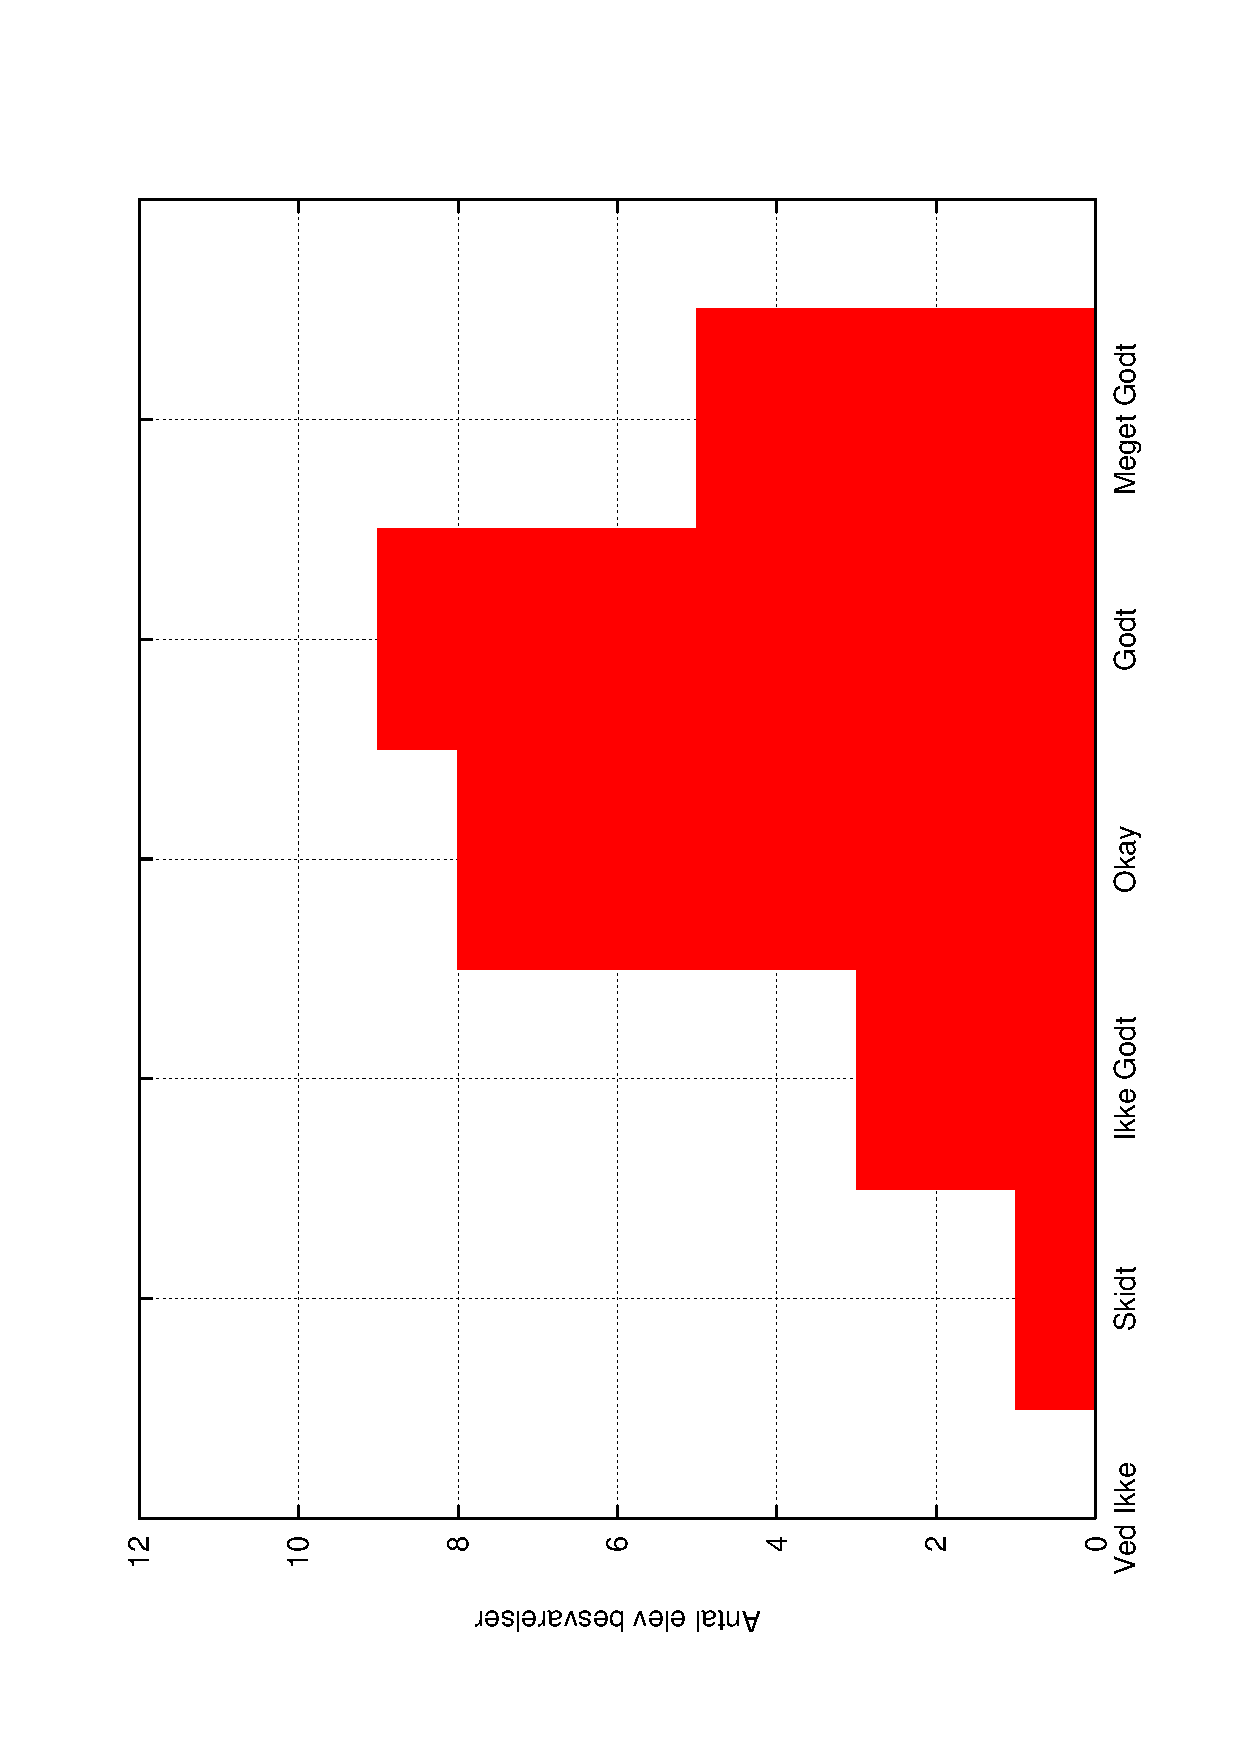
\includegraphics[width=.5\textwidth,angle=-90]{enepar}
	\caption{Ene-/pararbejde}
\end{figure}

\begin{figure}[h!]
	\centering
	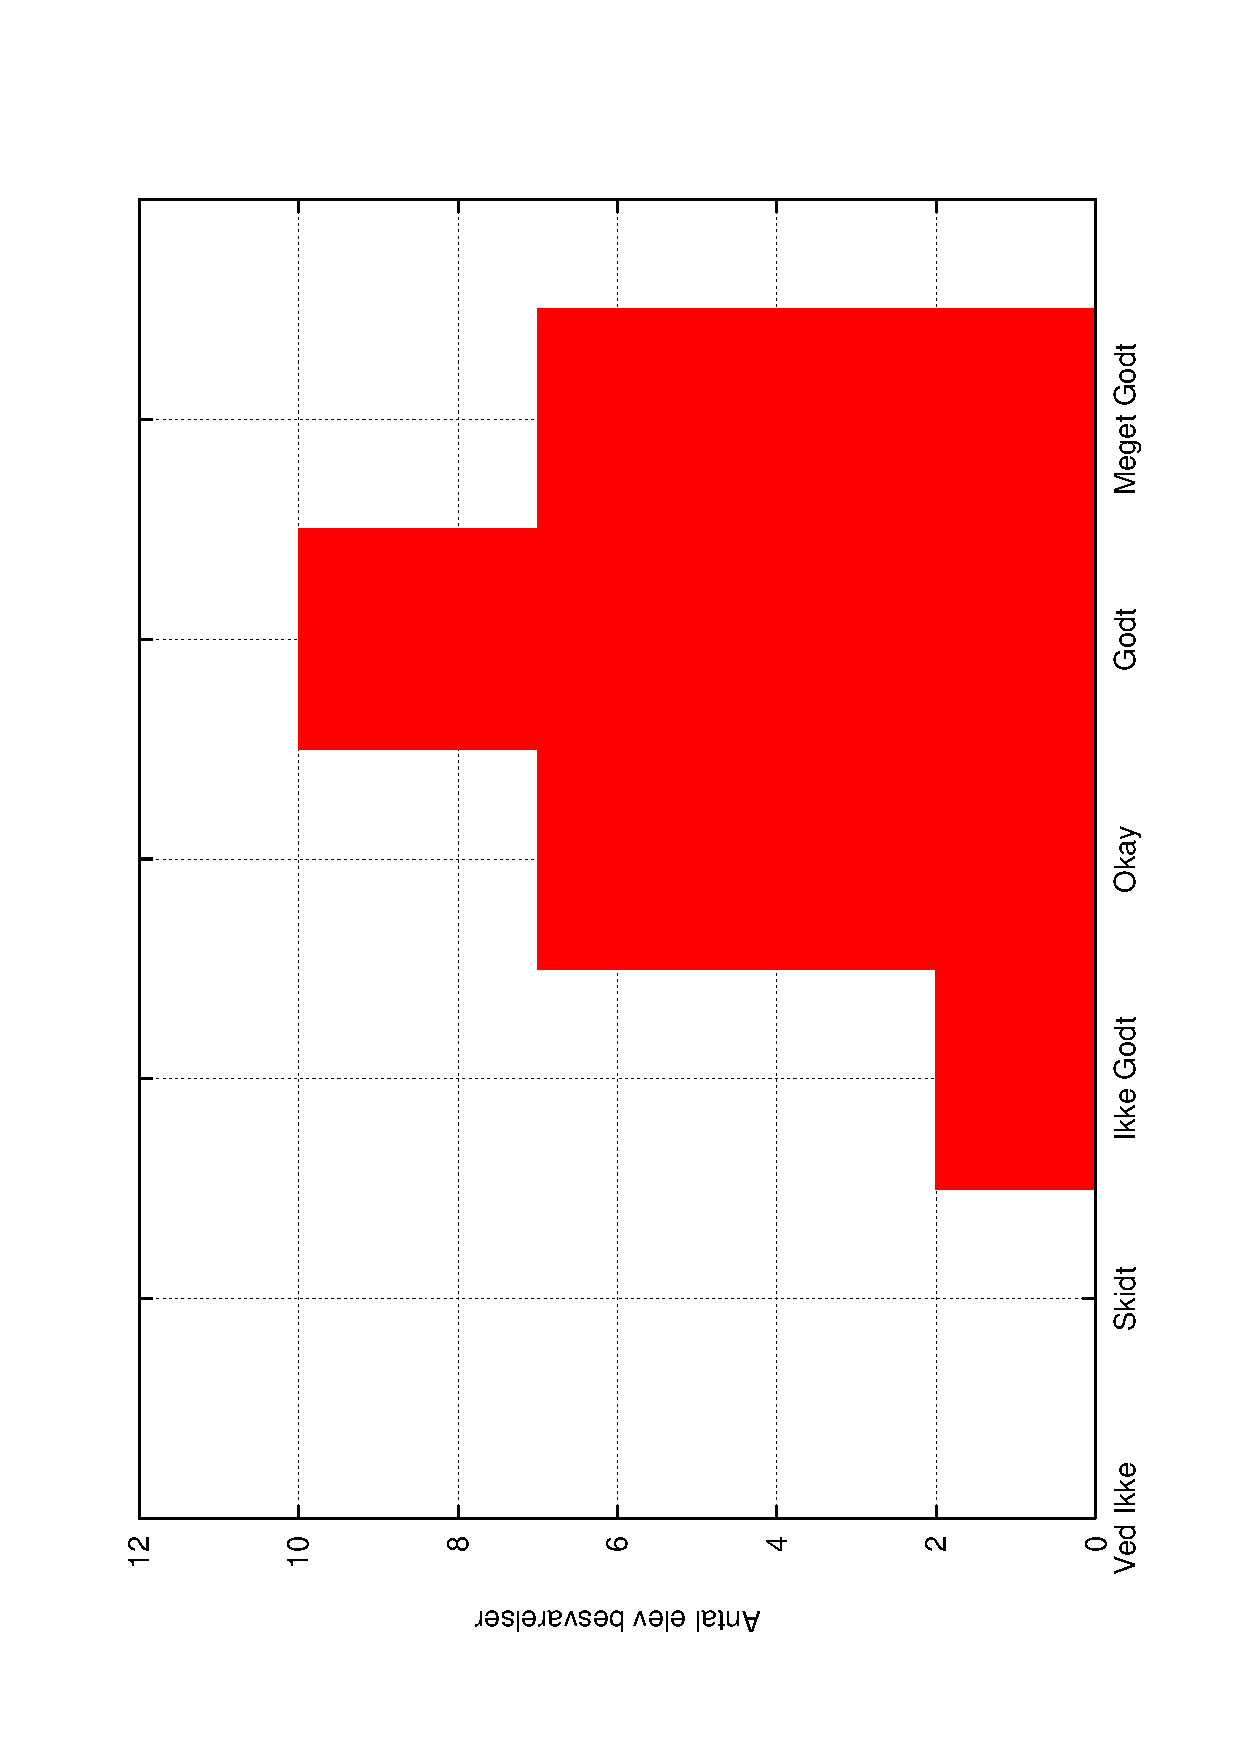
\includegraphics[width=.5\textwidth,angle=-90]{gruppe}
	\caption{Gruppearbejde}
\end{figure}

\begin{figure}[h!]
	\centering
	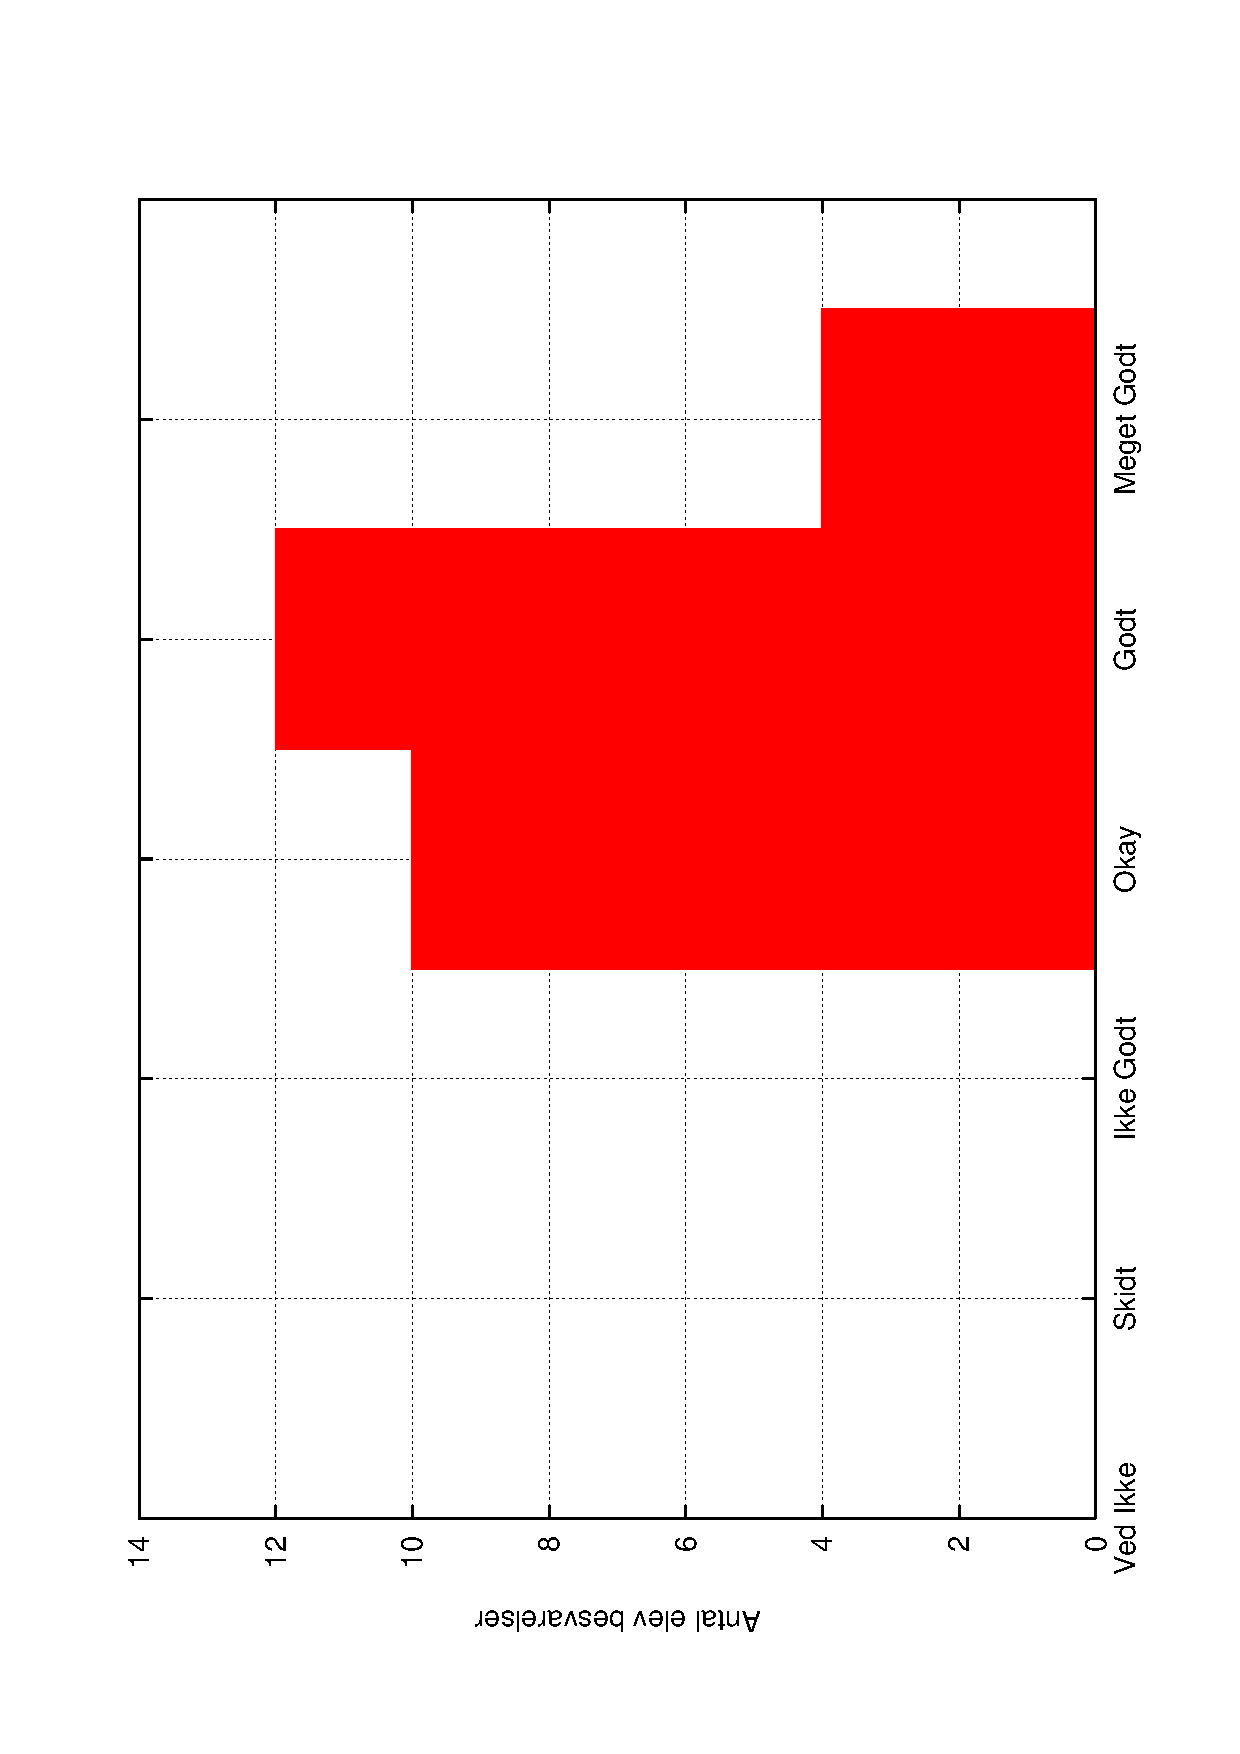
\includegraphics[width=.5\textwidth,angle=-90]{matrix}
	\caption{arbejde i Matrix grupper}
\end{figure}

\begin{figure}[h!]
	\centering
	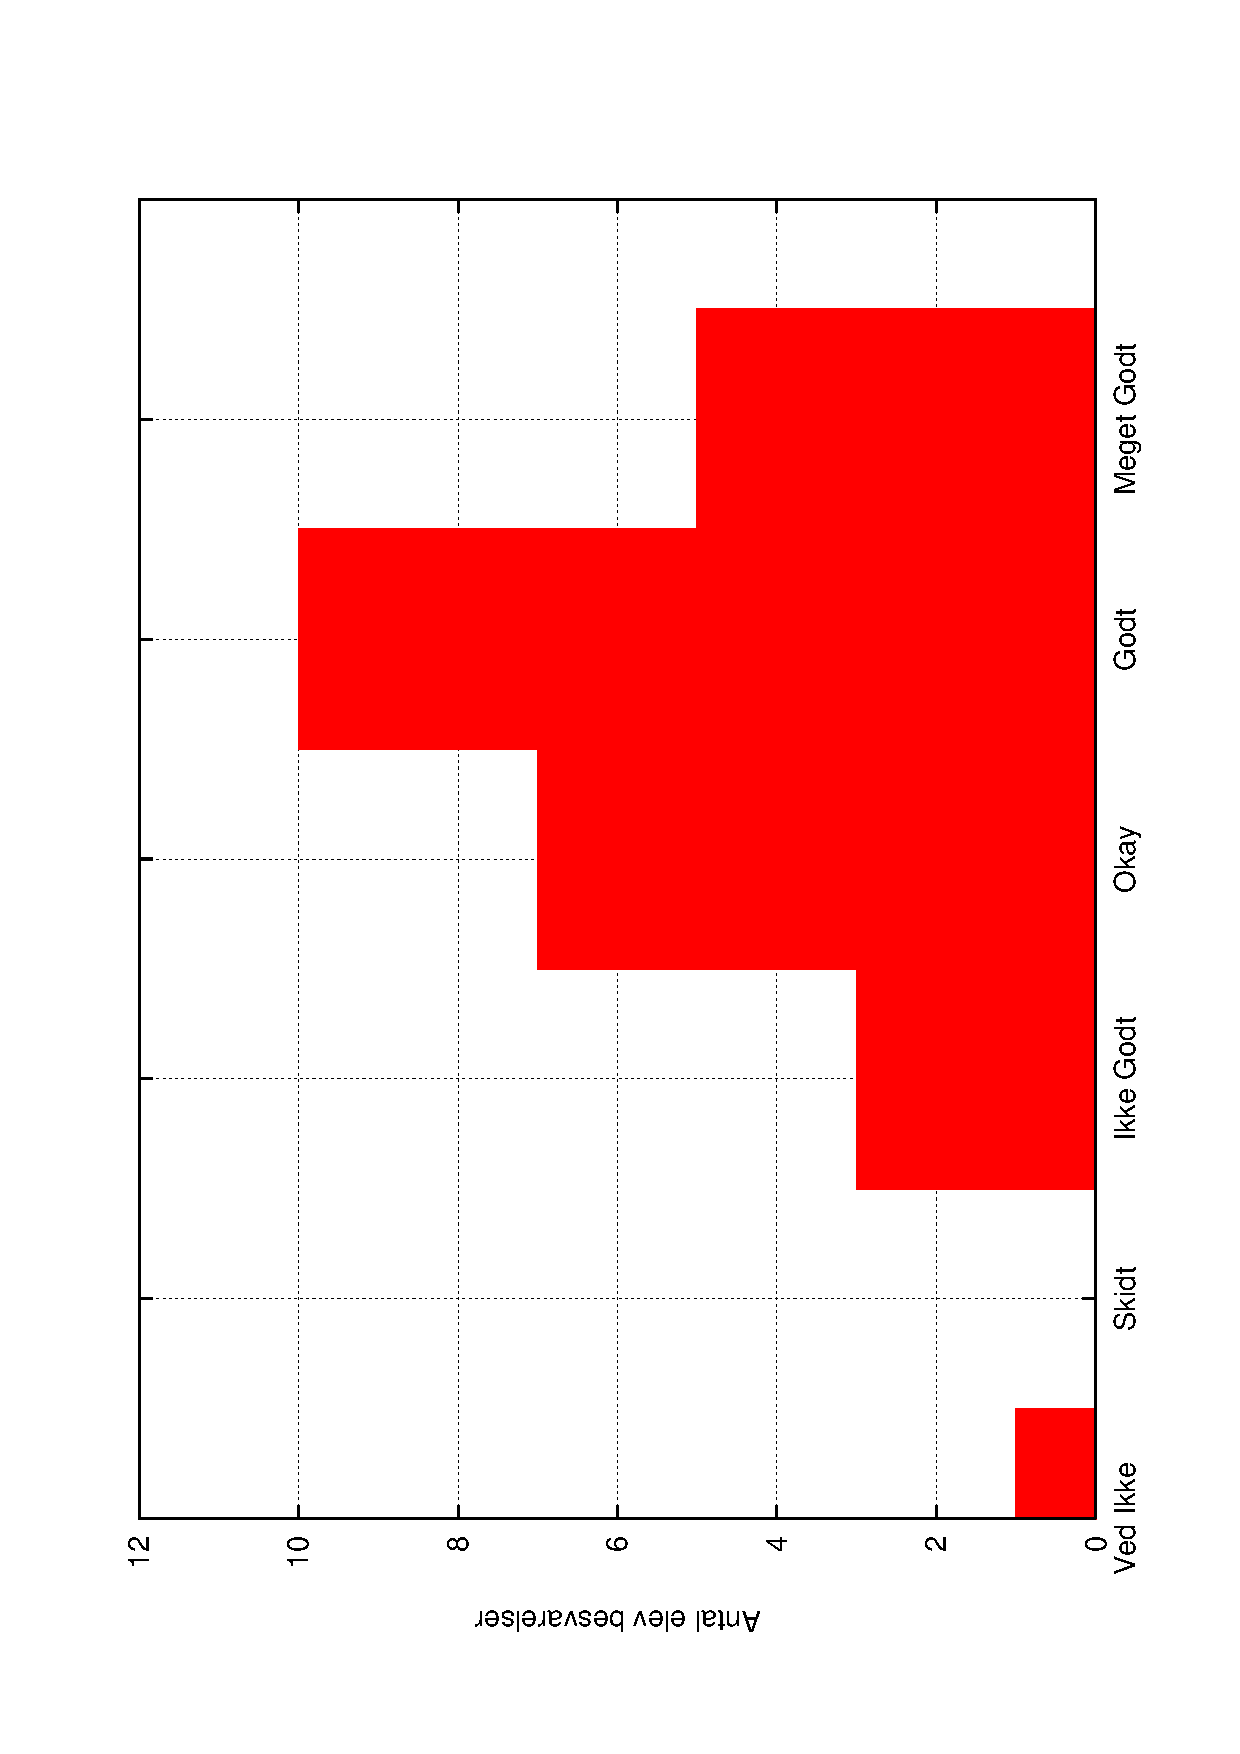
\includegraphics[width=.5\textwidth,angle=-90]{tavle}
	\caption{L�restyrret undervisning / Tavle undervisning}
\end{figure}

\begin{figure}[h!]
	\centering
	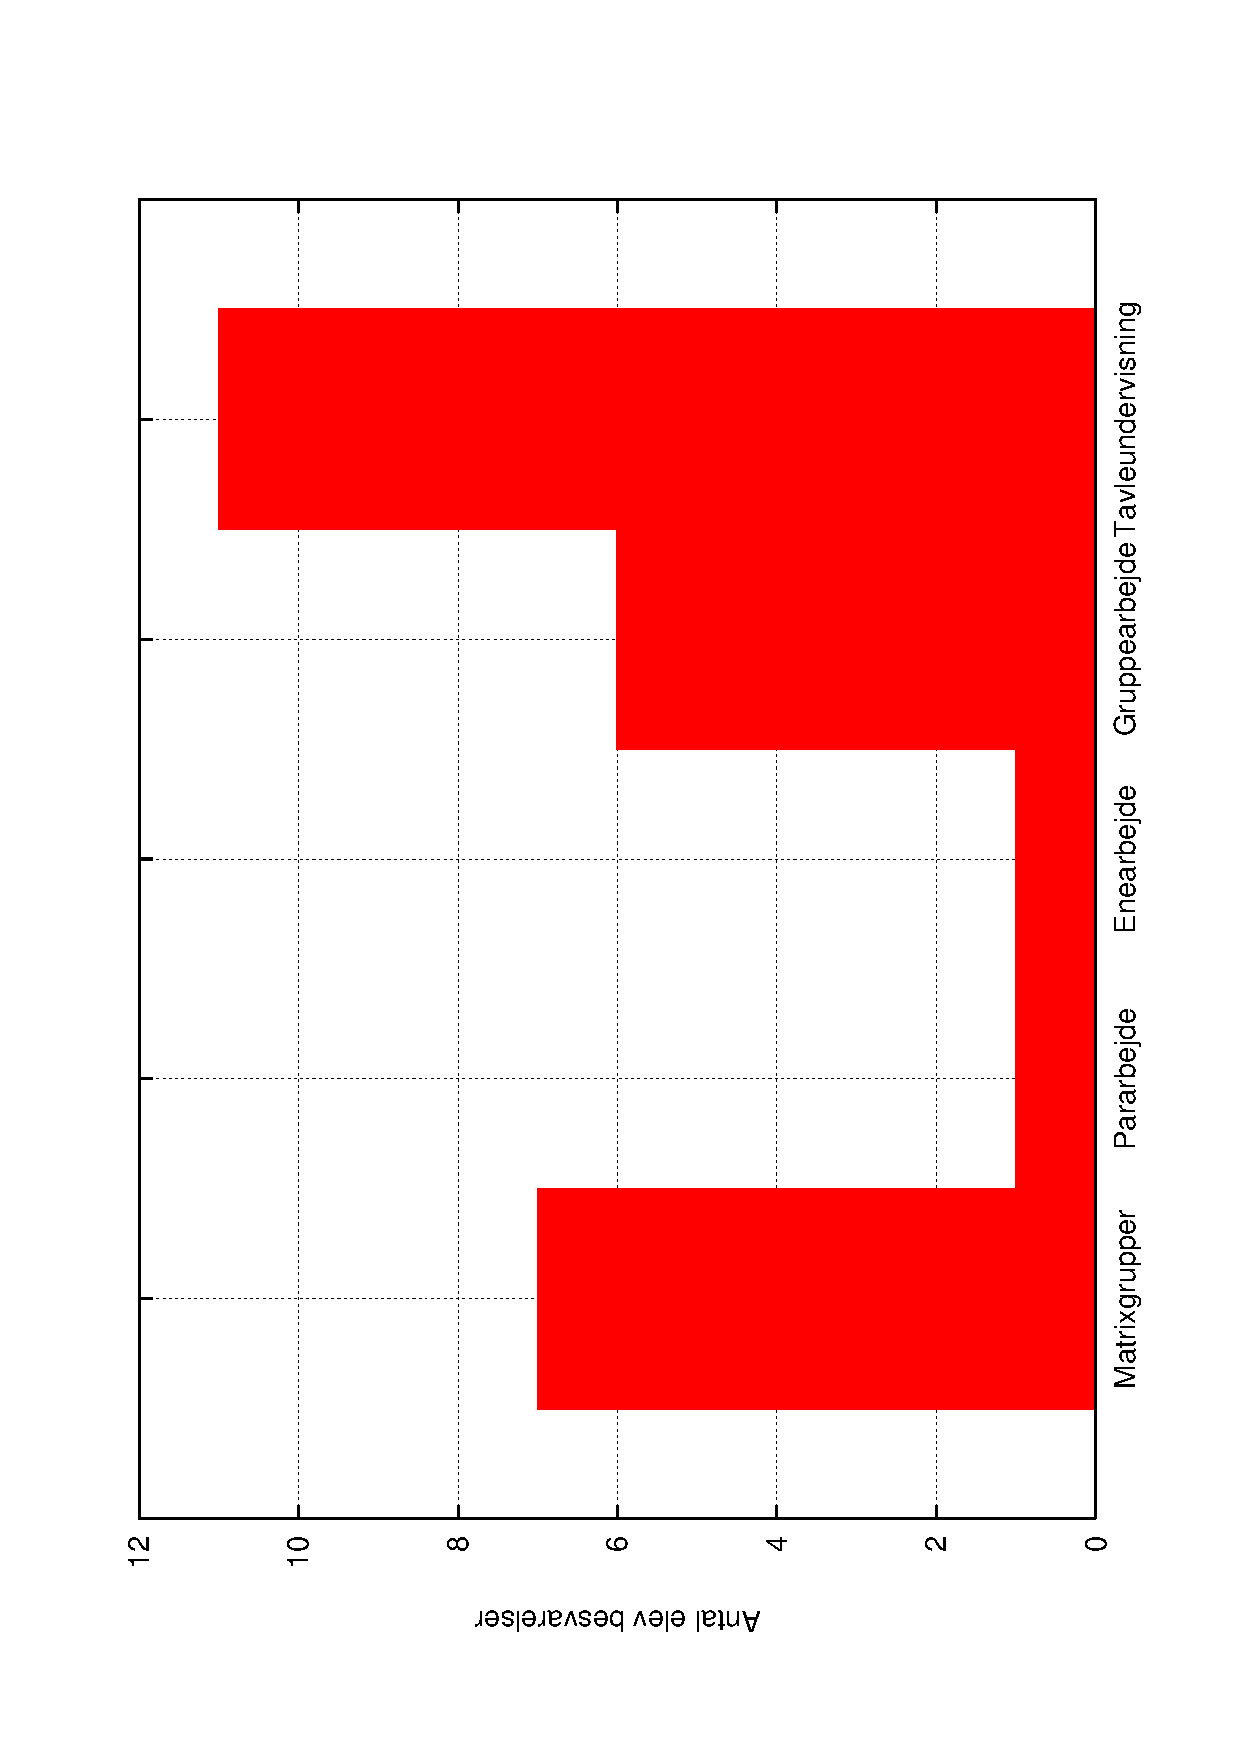
\includegraphics[width=.5\textwidth,angle=-90]{type}
	\caption{Foretrukket undervisnings type}
\end{figure}

\begin{figure}[h!]
	\centering
	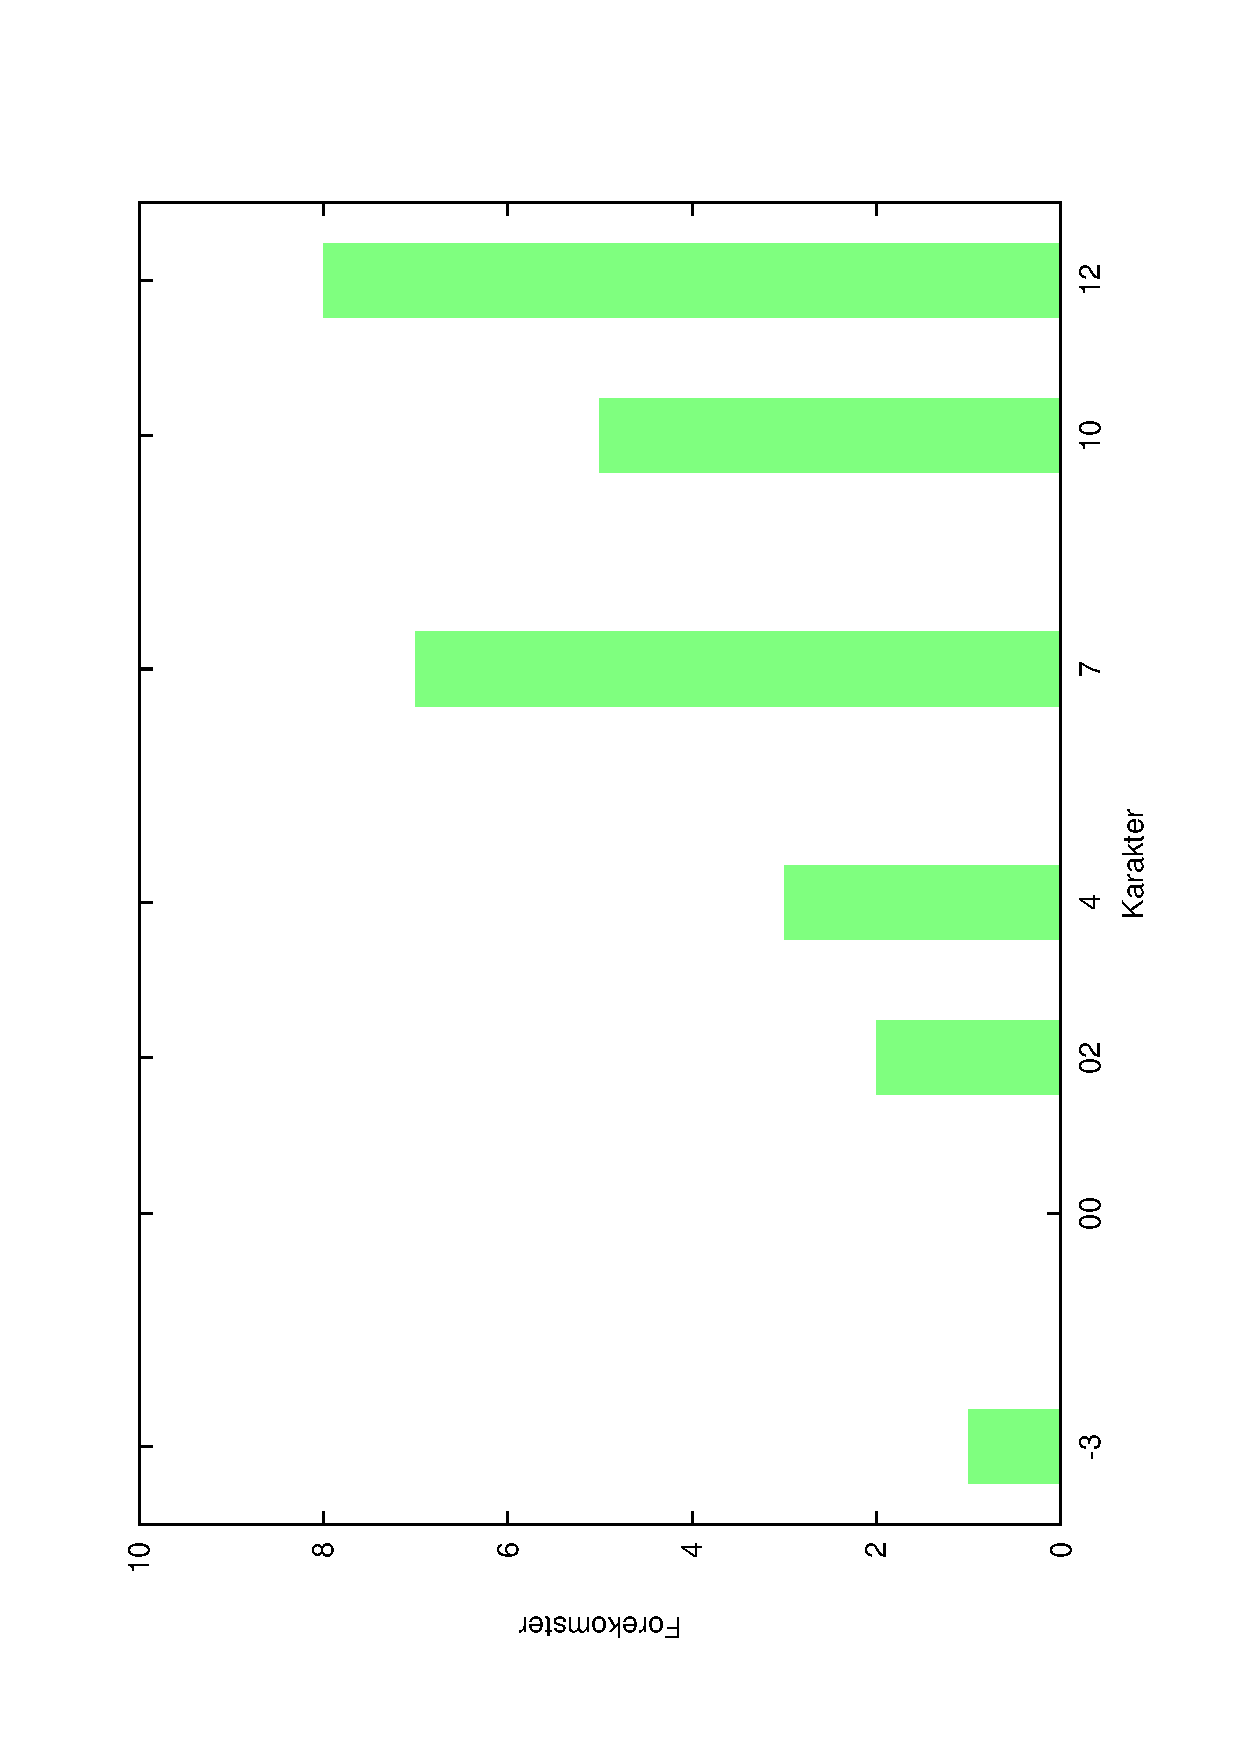
\includegraphics[width=.5\textwidth,angle=-90]{Verdensbilleder}
	\caption{Karakterfordeling for rapporter over forl�bet i klassen 1.m}
\end{figure}